\documentclass[]{article}
\usepackage{lmodern}
\usepackage{amssymb,amsmath}
\usepackage{ifxetex,ifluatex}
\usepackage{fixltx2e} % provides \textsubscript
\ifnum 0\ifxetex 1\fi\ifluatex 1\fi=0 % if pdftex
  \usepackage[T1]{fontenc}
  \usepackage[utf8]{inputenc}
\else % if luatex or xelatex
  \ifxetex
    \usepackage{mathspec}
  \else
    \usepackage{fontspec}
  \fi
  \defaultfontfeatures{Ligatures=TeX,Scale=MatchLowercase}
\fi
% use upquote if available, for straight quotes in verbatim environments
\IfFileExists{upquote.sty}{\usepackage{upquote}}{}
% use microtype if available
\IfFileExists{microtype.sty}{%
\usepackage{microtype}
\UseMicrotypeSet[protrusion]{basicmath} % disable protrusion for tt fonts
}{}
\usepackage[margin=1in]{geometry}
\usepackage{hyperref}
\hypersetup{unicode=true,
            pdftitle={Laborator 7},
            pdfborder={0 0 0},
            breaklinks=true}
\urlstyle{same}  % don't use monospace font for urls
\usepackage{color}
\usepackage{fancyvrb}
\newcommand{\VerbBar}{|}
\newcommand{\VERB}{\Verb[commandchars=\\\{\}]}
\DefineVerbatimEnvironment{Highlighting}{Verbatim}{commandchars=\\\{\}}
% Add ',fontsize=\small' for more characters per line
\usepackage{framed}
\definecolor{shadecolor}{RGB}{248,248,248}
\newenvironment{Shaded}{\begin{snugshade}}{\end{snugshade}}
\newcommand{\KeywordTok}[1]{\textcolor[rgb]{0.13,0.29,0.53}{\textbf{#1}}}
\newcommand{\DataTypeTok}[1]{\textcolor[rgb]{0.13,0.29,0.53}{#1}}
\newcommand{\DecValTok}[1]{\textcolor[rgb]{0.00,0.00,0.81}{#1}}
\newcommand{\BaseNTok}[1]{\textcolor[rgb]{0.00,0.00,0.81}{#1}}
\newcommand{\FloatTok}[1]{\textcolor[rgb]{0.00,0.00,0.81}{#1}}
\newcommand{\ConstantTok}[1]{\textcolor[rgb]{0.00,0.00,0.00}{#1}}
\newcommand{\CharTok}[1]{\textcolor[rgb]{0.31,0.60,0.02}{#1}}
\newcommand{\SpecialCharTok}[1]{\textcolor[rgb]{0.00,0.00,0.00}{#1}}
\newcommand{\StringTok}[1]{\textcolor[rgb]{0.31,0.60,0.02}{#1}}
\newcommand{\VerbatimStringTok}[1]{\textcolor[rgb]{0.31,0.60,0.02}{#1}}
\newcommand{\SpecialStringTok}[1]{\textcolor[rgb]{0.31,0.60,0.02}{#1}}
\newcommand{\ImportTok}[1]{#1}
\newcommand{\CommentTok}[1]{\textcolor[rgb]{0.56,0.35,0.01}{\textit{#1}}}
\newcommand{\DocumentationTok}[1]{\textcolor[rgb]{0.56,0.35,0.01}{\textbf{\textit{#1}}}}
\newcommand{\AnnotationTok}[1]{\textcolor[rgb]{0.56,0.35,0.01}{\textbf{\textit{#1}}}}
\newcommand{\CommentVarTok}[1]{\textcolor[rgb]{0.56,0.35,0.01}{\textbf{\textit{#1}}}}
\newcommand{\OtherTok}[1]{\textcolor[rgb]{0.56,0.35,0.01}{#1}}
\newcommand{\FunctionTok}[1]{\textcolor[rgb]{0.00,0.00,0.00}{#1}}
\newcommand{\VariableTok}[1]{\textcolor[rgb]{0.00,0.00,0.00}{#1}}
\newcommand{\ControlFlowTok}[1]{\textcolor[rgb]{0.13,0.29,0.53}{\textbf{#1}}}
\newcommand{\OperatorTok}[1]{\textcolor[rgb]{0.81,0.36,0.00}{\textbf{#1}}}
\newcommand{\BuiltInTok}[1]{#1}
\newcommand{\ExtensionTok}[1]{#1}
\newcommand{\PreprocessorTok}[1]{\textcolor[rgb]{0.56,0.35,0.01}{\textit{#1}}}
\newcommand{\AttributeTok}[1]{\textcolor[rgb]{0.77,0.63,0.00}{#1}}
\newcommand{\RegionMarkerTok}[1]{#1}
\newcommand{\InformationTok}[1]{\textcolor[rgb]{0.56,0.35,0.01}{\textbf{\textit{#1}}}}
\newcommand{\WarningTok}[1]{\textcolor[rgb]{0.56,0.35,0.01}{\textbf{\textit{#1}}}}
\newcommand{\AlertTok}[1]{\textcolor[rgb]{0.94,0.16,0.16}{#1}}
\newcommand{\ErrorTok}[1]{\textcolor[rgb]{0.64,0.00,0.00}{\textbf{#1}}}
\newcommand{\NormalTok}[1]{#1}
\usepackage{graphicx,grffile}
\makeatletter
\def\maxwidth{\ifdim\Gin@nat@width>\linewidth\linewidth\else\Gin@nat@width\fi}
\def\maxheight{\ifdim\Gin@nat@height>\textheight\textheight\else\Gin@nat@height\fi}
\makeatother
% Scale images if necessary, so that they will not overflow the page
% margins by default, and it is still possible to overwrite the defaults
% using explicit options in \includegraphics[width, height, ...]{}
\setkeys{Gin}{width=\maxwidth,height=\maxheight,keepaspectratio}
\IfFileExists{parskip.sty}{%
\usepackage{parskip}
}{% else
\setlength{\parindent}{0pt}
\setlength{\parskip}{6pt plus 2pt minus 1pt}
}
\setlength{\emergencystretch}{3em}  % prevent overfull lines
\providecommand{\tightlist}{%
  \setlength{\itemsep}{0pt}\setlength{\parskip}{0pt}}
\setcounter{secnumdepth}{5}
% Redefines (sub)paragraphs to behave more like sections
\ifx\paragraph\undefined\else
\let\oldparagraph\paragraph
\renewcommand{\paragraph}[1]{\oldparagraph{#1}\mbox{}}
\fi
\ifx\subparagraph\undefined\else
\let\oldsubparagraph\subparagraph
\renewcommand{\subparagraph}[1]{\oldsubparagraph{#1}\mbox{}}
\fi

%%% Use protect on footnotes to avoid problems with footnotes in titles
\let\rmarkdownfootnote\footnote%
\def\footnote{\protect\rmarkdownfootnote}

%%% Change title format to be more compact
\usepackage{titling}

% Create subtitle command for use in maketitle
\newcommand{\subtitle}[1]{
  \posttitle{
    \begin{center}\large#1\end{center}
    }
}

\setlength{\droptitle}{-2em}

  \title{Laborator 7}
    \pretitle{\vspace{\droptitle}\centering\huge}
  \posttitle{\par}
  \subtitle{Legea Numerelor Mari și Teorema Limită Centrală}
  \author{}
    \preauthor{}\postauthor{}
    \date{}
    \predate{}\postdate{}
  
\usepackage{booktabs}
\usepackage{longtable}
\usepackage{framed,color}
\definecolor{shadecolor}{RGB}{248, 248, 248}
\definecolor{shadecolor1}{RGB}{216,225,235}
\definecolor{framecolor}{RGB}{16,111,124}%108,123,13

%\definecolor{shadecolor}{RGB}{226, 255, 241}
% \definecolor{shadecolor1}{RGB}{217,225,199}
% \definecolor{framecolor}{RGB}{60,179,113}

%%%%%%%%%%%%%%%%%%%%%%
\ifxetex
  \usepackage{letltxmacro}
  \setlength{\XeTeXLinkMargin}{1pt}
  \LetLtxMacro\SavedIncludeGraphics\includegraphics
  \def\includegraphics#1#{% #1 catches optional stuff (star/opt. arg.)
    \IncludeGraphicsAux{#1}%
  }%
  \newcommand*{\IncludeGraphicsAux}[2]{%
    \XeTeXLinkBox{%
      \SavedIncludeGraphics#1{#2}%
    }%
  }%
\fi

\newenvironment{frshaded*}{%
  \def\FrameCommand{\fboxrule=\FrameRule\fboxsep=\FrameSep \fcolorbox{framecolor}{shadecolor1}}%
  \MakeFramed {\advance\hsize-\width \FrameRestore}}%
{\endMakeFramed}

\newenvironment{rmdblock}[1]
  {\begin{frshaded*}
  \begin{itemize}
  \renewcommand{\labelitemi}{
    \raisebox{-.7\height}[0pt][0pt]{
      {\setkeys{Gin}{width=2em,keepaspectratio}\includegraphics{images/icons/#1}}
    }
  }
  \item
  }
  {
  \end{itemize}
  \end{frshaded*}
  }
  
%%%%%%%%%%%%%%%
% definitions.
% -------------------
\usepackage{marginnote}
% \renewcommand*{\marginnotevadjust}{40pt}
% \renewcommand{\marginnotevadjust}{0pt}
% \renewcommand{\marginfont}{\noindent\rule{0pt}{0.7\baselineskip}\tiny}

\newtheorem{proposition}{Proposition}[section]
\newtheorem{lemma}[proposition]{Lemma}
\newtheorem{corollary}[proposition]{Corollary}
\newtheorem{theorem}[proposition]{Theorem}

\newcounter{exo}[section]
\newcommand{\enonce}[2]{\refstepcounter{proposition}\hypertarget{exo:#1}{}\label{exo:#1}{\scriptsize\;\textbf{Ex.}~\ref{exo:#1}}}

\reversemarginpar
\setlength{\marginparwidth}{1.2cm}
% 
% \newcommand{\enonce}[2]{\refstepcounter{proposition}\hypertarget{exo:#1}{}\label{exo:#1}{\noindent\color{black}\normalsize\bf Exercice \ref{exo:#1}}\ \  #2\vspace{1mm}\hrule\vspace{1mm} \color{black}\normalsize}


%%%%%%%%%%%%%%%

% \newenvironment{rmdcaution}
%   {\begin{rmdblock}{caution}}
%   {\end{rmdblock}}

% \newenvironment{rmdinsight}
%   {\begin{rmdblock}{insight}}
%   {\end{rmdblock}}

\newenvironment{rmdexercise}
  {\begin{rmdblock}{exercise}}
  {\end{rmdblock}}

% \newenvironment{rmdexercise_tex}
%   {\begin{rmdblock}{exercise}}
%   {\end{rmdblock}}
  
% \newenvironment{rmdtip}
%   {\begin{rmdblock}{tip}}
%   {\end{rmdblock}}


%%%%%%%%%%%%%%%%%%%%%%%%%%%%%%%%%%%%%%%%%%%%%%%%%%%%%%%%%%%%%%%%%%%%%%%%%%%%%%%%%%%%%%%%%%%%%%%%%%%%%%%%%%%%%%%%%%%%%
%%%%%%%%%%% For insight block %%%%%%%%%%%%%%%%%%%%%%%%%%
\definecolor{shadecolor_insight}{RGB}{223,240,216}
\definecolor{framecolor_insight}{RGB}{136,193,137}

%\definecolor{shadecolor_insight}{RGB}{217,225,199}
%\definecolor{framecolor_insight}{RGB}{60,179,113}

\newenvironment{frshaded_insight*}{%
  \def\FrameCommand{\fboxrule=\FrameRule\fboxsep=\FrameSep \fcolorbox{framecolor_insight}{shadecolor_insight}}%
  \MakeFramed {\advance\hsize-\width \FrameRestore}}%
{\endMakeFramed}

\newenvironment{rmdblock_insight}[1]
  {\begin{frshaded_insight*}
  \begin{itemize}
  \renewcommand{\labelitemi}{
    \raisebox{-.7\height}[0pt][0pt]{
      {\setkeys{Gin}{width=2em,keepaspectratio}\includegraphics{images/icons/#1}}
    }
  }
  \item
  }
  {
  \end{itemize}
  \end{frshaded_insight*}
  }

\newenvironment{rmdinsight}
  {\begin{rmdblock_insight}{insight}}
  {\end{rmdblock_insight}}

%%%%%%%%%%% For caution block %%%%%%%%%%%%%%%%%%%%%%%%%%
\definecolor{shadecolor_caution}{RGB}{250,250,250}
\definecolor{framecolor_caution}{RGB}{242,129,67}%193,75,34

\newenvironment{frshaded_caution*}{%
  \def\FrameCommand{\fboxrule=\FrameRule\fboxsep=\FrameSep \fcolorbox{framecolor_caution}{shadecolor_caution}}%
  \MakeFramed {\advance\hsize-\width \FrameRestore}}%
{\endMakeFramed}

\newenvironment{rmdblock_caution}[1]
  {\begin{frshaded_caution*}
  \begin{itemize}
  \renewcommand{\labelitemi}{
    \raisebox{-.7\height}[0pt][0pt]{
      {\setkeys{Gin}{width=2em,keepaspectratio}\includegraphics{images/icons/#1}}
    }
  }
  \item
  }
  {
  \end{itemize}
  \end{frshaded_caution*}
  }
  
\newenvironment{rmdcaution}
  {\begin{rmdblock_caution}{caution}}
  {\end{rmdblock_caution}}

%%%%%%%%%%% For tip block %%%%%%%%%%%%%%%%%%%%%%%%%%
\definecolor{shadecolor_tip}{RGB}{250,250,250}
\definecolor{framecolor_tip}{RGB}{33,153,195}

\newenvironment{frshaded_tip*}{%
  \def\FrameCommand{\fboxrule=\FrameRule\fboxsep=\FrameSep \fcolorbox{framecolor_tip}{shadecolor_tip}}%
  \MakeFramed {\advance\hsize-\width \FrameRestore}}%
{\endMakeFramed}

\newenvironment{rmdblock_tip}[1]
  {\begin{frshaded_tip*}
  \begin{itemize}
  \renewcommand{\labelitemi}{
    \raisebox{-.7\height}[0pt][0pt]{
      {\setkeys{Gin}{width=2em,keepaspectratio}\includegraphics{images/icons/#1}}
    }
  }
  \item
  }
  {
  \end{itemize}
  \end{frshaded_tip*}
  }
  
\newenvironment{rmdtip}
  {\begin{rmdblock_tip}{tip}}
  {\end{rmdblock_tip}}

%%%%%%%%%%%%%%%%%%%%%%%%%%%%%%%%%%%%%%%%%%%%%%%%%%%%%%%%%%%%%%%%%%%%%%%%%%%%%%%%%%%%%%%%%%%%%%%%%%%%%%%%%%%%%%%%%%%%%
\usepackage{subfigure}
\usepackage{booktabs}
\usepackage{slashbox}
\usepackage{color}
%%%%%%%%%%%%%%%%%%%%%%%%%%%%%%%%%%%%%%%%%
\definecolor{linkcol}{rgb}{0,0,0.4}
\definecolor{citecol}{rgb}{0.5,0,0}

% Change this to change the informations included in the pdf file
% \usepackage[pagebackref]{hyperref}
% \usepackage[verbose]{backref}
\usepackage[hyperpageref]{backref}
% \backrefsetup{verbose=false}
% \PassOptionsToPackage{pagebackref}{hyperref}
% See hyperref documentation for information on those parameters

\hypersetup
{
bookmarksopen=true,
pdftitle="Curs Probabilitati si Statistica",
pdfauthor="Alexandru Amarioarei",
pdfsubject="Curs Probabilitati si Statistica", %subject of the document
pdfmenubar=true, %menubar shown
pdfhighlight=/O, %effect of clicking on a link
colorlinks=true, %couleurs sur les liens hypertextes
pdfpagemode=None, %aucun mode de page
pdfpagelayout=SinglePage, %ouverture en simple page
pdffitwindow=true, %pages ouvertes entierement dans toute la fenetre
linkcolor=linkcol, %couleur des liens hypertextes internes
citecolor=citecol, %couleur des liens pour les citations
urlcolor=linkcol %couleur des liens pour les url
}


% set the back references
\renewcommand*{\backref}[1]{}
\renewcommand*{\backreftwosep}{ și~} % inserted between entries 
                              % in a list of two entries, 
                              % default is " and~".
\renewcommand*{\backreflastsep}{ și~} % inserted between the last 
                               % two entries of a list with more
                               % than two entries, default is ", and~".
\renewcommand*{\backrefalt}[4]{%
    \ifcase #1 (Necitat.)%
    \or        (Citat la pagina~#2.)%
    \else      (Citat la paginile~#2.)%
    \fi}

%%%%%%%%%%%%%%%%%%%%%%%%%%%%%%%%%%%%%%%%%%%%%%%%%%%%%%%%%%%%%%%%%%%%%%%%%%%%%%%%%%%%%%%%%%%%%%%%%%%%%%%%%%%%%%%%%%%%%
%CITEVA DEFINITII
\def\om{\omega}
\def\Om{\Omega}
\def\et{\eta}
\def\td{\tilde{\delta}}
\def\m{{\mu}}
\def\n{{\nu}}
\def\k{{\kappa}}
\def\l{{\lambda}}
\def\L{{\Lambda}}
\def\g{{\gamma}}
\def\a{{\alpha}}
\def\e{{\varepsilon}}
\def\b{{\beta}}
\def\G{{\Gamma}}
\def\d{{\delta}}
\def\D{{\Delta}}
\def\t{{\theta}}
\def\s{{\sigma}}
\def\S{{\Sigma}}
\def\z{{\zeta}}
\def\qed{\hfill\Box}
\def\ds{\displaystyle}
\def\mc{\mathcal}
%%%%%%%%%%%%%%%%%%%%%%%%%%%%%%%%%%%%%%%%%%%%%%%%%%%%%%%%%%%%%%%%%%%%%%%%%%%%%%%%%%%%%%%%%%%%%%%%%%%%%%%%%%%%%%%%%%%%%%
\def\1{{\mathbf 1}}
\def\CC{{\mathbb C}}
\def\VV{{\mathbb V}}
\def\RR{{\mathbb R}}
\def\QQ{{\mathbb Q}}
\def\ZZ{{\mathbb Z}}
\def\PP{{\mathbb P}}
\def\EE{{\mathbb E}}
\def\NN{{\mathbb N}}
\def\FF{{\mathbb F}}
%\def\SS{{\mathbb S}}
\def\MA{{\mathcal A}}
\def\MO{{\mathcal O}}
\def\MF{{\mathcal F}}
\def\ME{{\mathcal E}}
\def\MR{{\mathcal R}}
\def\MB{{\mathcal B}}
\def\MM{{\mathcal M}}
\def\MN{{\mathcal N}}
\def\MU{{\mathcal U}}
\def\MP{{\mathcal P}}
\def\MS{{\mathcal S}}
\def\MBS{{\mathbf S}}
\def\MX{{\bm{ \mathscr X}}}

% independent sign
\newcommand\independent{\protect\mathpalette{\protect\independenT}{\perp}}
\def\independenT#1#2{\mathrel{\rlap{$#1#2$}\mkern2mu{#1#2}}}

\renewcommand\tablename{Tab.}
\renewcommand{\figurename}{Fig.}
\renewcommand\refname{Referințe}

%%%%%%%%%%%%%%%%%%%%%%%%%%%%%%%%%%%%%%%%%%%%%%%%%%%%%%%%%%%%%%%%%%%%%%%%%%%%%%%%%%%%%%%%%%%%%%%%%%%%%%%%%%%%%%%%%%%%%
%Header and Footer
\usepackage{fancyhdr}

\pagestyle{fancy}
\fancyhf{}
\rhead{Universitatea din Bucure\c sti\\ Facultatea de Matematic\u a \c si Informatic\u a}
% \lhead{\textit{Curs}: Tehnici alternative în predarea matematicii (2018)\\ \textit{Instructori}: A. Am\u arioarei, M. Patriche}
\lhead{\textit{Curs}: Probabilități și Statistică (2018-2019)\\ \textit{Instructor}: A. Am\u arioarei}
\rfoot{Pagina \thepage}
\lfoot{Grupele: 241, 242, 243, 244}
%%%%%%%%%%%%%%%%%%%%%%%%%%%%%%%%%%%%%%%
%%%%%%%%%%%%%%%%%%%%%%%%%%%%%%%%%%%%%%%
\usepackage{pifont}% http://ctan.org/pkg/pifont
\newcommand{\cmark}{\ding{51}}%
\newcommand{\xmark}{\ding{55}}%
\usepackage{booktabs}
\usepackage{longtable}
\usepackage{array}
\usepackage{multirow}
\usepackage[table]{xcolor}
\usepackage{wrapfig}
\usepackage{float}
\usepackage{colortbl}
\usepackage{pdflscape}
\usepackage{tabu}
\usepackage{threeparttable}
\usepackage{threeparttablex}
\usepackage[normalem]{ulem}
\usepackage{makecell}

\begin{document}
\maketitle

%%%%%%%%%%%%%%%%%%%%%%%%
\thispagestyle{fancy}

Obiectivul acestui laborator este de a prezenta noțiunea de convergență
în probabilitate și convergență în repartiție precum și a \emph{Legii
Numerelor Mari} (versiunea slabă) și a \emph{Teoremei Limită Centrale}.

\section{Ilustrarea Legii Numerelor
Mari}\label{ilustrarea-legii-numerelor-mari}

\subsection{Convergența în
probabilitate}\label{convergenta-in-probabilitate}

Fie \(X_n, n\geq 1\) și \(X\) variabile aleatoare definite pe câmpul de
probabilitate \((\Omega, \mathcal{F}, \mathbb{P})\). Spunem că un șirul
de variabile aleatoare \((X_n)_n\) converge în probabilitate la
variabila aleatoare \(X\), și notăm \(X_n\overset{\mathbb{P}}{\to}X\),
dacă pentru orice \(\epsilon>0\) are loc

\[
  \mathbb{P}\left(\left|X_{n} - X\right| > \epsilon\right) \overset{n\to\infty}{\longrightarrow} 0. 
\]

De asemenea putem observa că \(X_n\overset{\mathbb{P}}{\to}X\) dacă și
numai dacă \(X_n-X\overset{\mathbb{P}}{\to}0\). Pentru a ilustra grafic
acest tip de convergență\footnote{Pentru alte moduri de convergență și
  ilustrarea lor grafică se poate consulta lucrarea: Pierre LAFAYE DE
  MICHEAUX și Benoit LIQUET \emph{Understanding Convergence Concepts: A
  Visual-Minded and Graphical Simulation-Based Approach}, The American
  Statistician, Vol. 63, No. 2, 2009} vom aproxima probabilitatea
\(\mathbb{P}(A_n)\), unde
\(A_n = \{\omega\in\Omega\,|\,\left|X_{n}(\omega) - X(\omega)\right| > \epsilon\}\),
folosind abordarea frecvenționistă. Aceasta presupune ca pentru \(n\)
dat să considerăm \(\omega_1, \ldots,\omega_M\in\Omega\), \(M\)
realizări ale experimentului (repetat în condiții identice) și să
folosim aproximarea

\[
  \mathbb{P}(A_n) \approx p_n(M) = \frac{\#\left\{j\in\{1,\ldots,M\}\,|\,\left|X_{n}(\omega_j) - X(\omega_j)\right| > \epsilon\right\}}{M}.
\]

Concret, în figura de mai jos, considerăm \(M = 30\) de repetiții ale
experimentului (avem \(M\) curbe) cu \(n = 5000\) de realizări ale unui
șir de variabile aleatoare \(X_k = \frac{Y_1+\cdots+Y_k}{k}\), cu
\(Y_i\) independente și repartizate \(\mathcal{U}[0,1]\), \(X = 0.5\) și
\(\epsilon = 0.01\). Pentru \(i\in\{500, 1500, 2500, 3500, 4500\}\) am
calculat și afișat frecvența de realizarea a evenimentului \(A_i\) (câte
din cele \(M\) curbe sunt în afara benzii \([-\epsilon, \epsilon]\)
pentru \(i\), fixat). Observăm că \(p_{500}(30) = 0.37\) și
\(p_{3500}(30) = 0.03\), convergența lui
\(p_n(M)\underset{n\to \infty}{\longrightarrow} 0\) implicând
convergența în probabilitate.

\begin{center}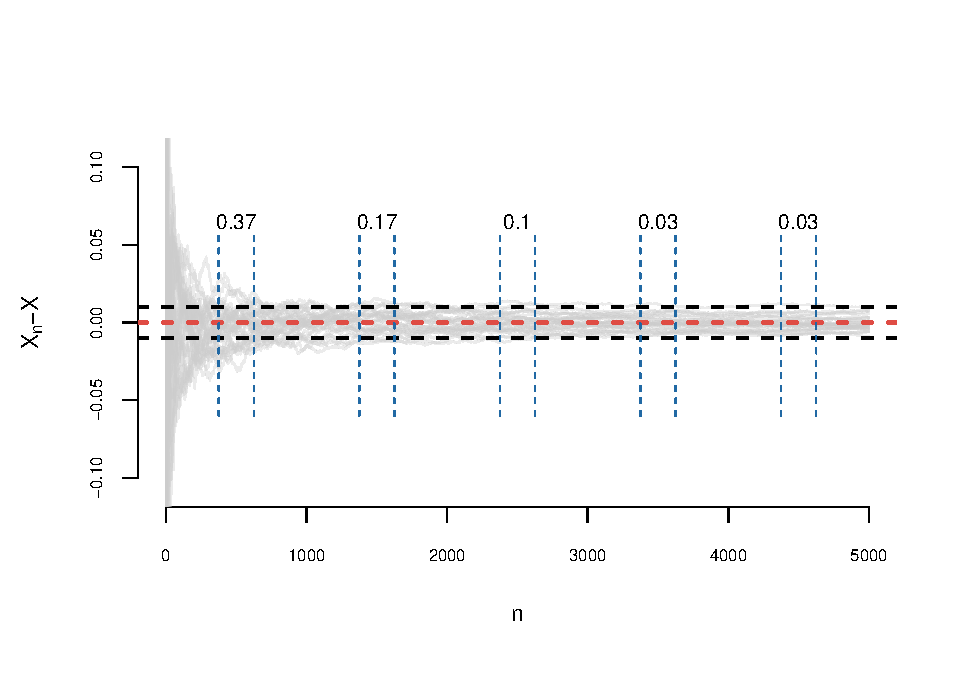
\includegraphics[width=0.7\linewidth]{Lab7_files/figure-latex/unnamed-chunk-3-1} \end{center}

\subsection{Legea numerelor mari (versiunea
slabă)}\label{legea-numerelor-mari-versiunea-slaba}

\begin{rmdinsight}
Fie \(X_1, X_2, \ldots\) un șir de variabile aleatoare independente și
indentic repartizate, de medie \(\mathbb{E}[X_1] = \mu<\infty\) și
varianță \(Var(X_1) = \sigma^2<\infty\). Atunci \(\forall \epsilon>0\)
avem

\[
  \mathbb{P}\left(\left|\frac{X_1+\cdots+X_n}{n} - \mu\right| > \epsilon\right) \overset{n\to\infty}{\longrightarrow} 0
\]

sau echivalent

\[
  \mathbb{P}\left(\left|\frac{X_1+\cdots+X_n}{n} - \mu\right| \leq \epsilon\right) \overset{n\to\infty}{\longrightarrow} 1
\]
\end{rmdinsight}

Notând \(\bar{X}_n = \frac{X_1+\cdots X_n}{n}\), \emph{Legea numerelor
mari (versiunea slabă)} afirmă că
\(\bar{X}_n\overset{\mathbb{P}}{\to}\mu\). Figura de mai jos ilustrează
această convergență pentru \(M = 100\) de traiectorii. În figura din
dreapta este ilustrată evoluția probabilității \(p_n\) pentru
\(n\in\{1,2,\ldots, N\}\).

\begin{center}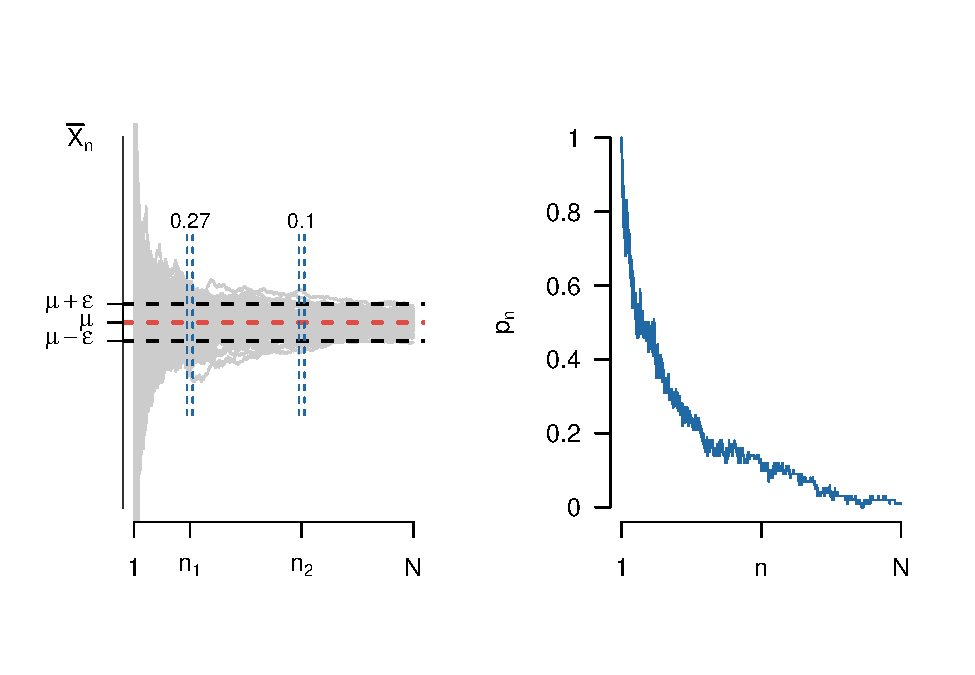
\includegraphics[width=0.8\linewidth]{Lab7_files/figure-latex/unnamed-chunk-5-1} \end{center}

\begin{rmdexercise}
Să presupunem că primim o monedă și ni se spune că aceasta aterizează pe
fața cap în \(48\%\) din cazuri. Vrem să testăm această afirmație.
Folosind \emph{Legea numerelor mari} și știind că vrem să fim siguri în
\(95\%\) din cazuri, ne întrebăm de câte ori trebuie să aruncăm moneda
pentru a verifica afirmația?
\end{rmdexercise}

Să presupunem că aruncăm moneda, independent, de \(n\) ori și fie
\(X_i\) rezultatul obținut la cea de-a \(i\)-a aruncare: \(X_i=1\) dacă
la a \(i\)-a aruncare am obținut cap și \(X_i = 0\) dacă am obținut
pajură. Avem că variabilele aleatoare \(X_1, X_2, \ldots, X_n\) sunt
independente și repartizare \(\mathcal{B}(p)\), cu \(p=0.48\) din
ipoteză.

De asemenea, observăm că \(\mathbb{E}[X_1]= \mu = 0.48\) și
\(Var(X_1) = \sigma^2 = p(1-p) = 0.2496\). Pentru testarea monedei
permitem o eroare \(\epsilon = 0.02\) ceea ce înseamnă că probabilitatea
ca moneda să aterizeze cap se află în intervalul \((0.46, 0.5)\). Din
\emph{Inegalitatea lui Cebîșev} avem că

\[
  \mathbb{P}\left(\left|\frac{X_1+\cdots+X_n}{n} - 0.48\right| >0.02\right)\leq \frac{Var(X_1)}{n\times(0.02)^2}, 
\]

de unde, având un grad de încredere de \(95\%\), vrem să determinăm pe
\(n\) pentru care

\[
  \frac{0.2496}{n\times(0.02)^2} = 0.05
\]

ceea ce implică \(n = 12480\).

\begin{rmdexercise}
Fie \(X_1,X_2,\dots,X_N\), \(N\) v.a. i.i.d. de lege
\(\mathcal{U}([0,1])\). Pentru \(1\leq n\leq N\), notăm cu
\(S_n=X_1+X_2+\cdots X_n\) șirul sumelor parțiale și \(\mu\) media legii
\(\mathcal{U}([0,1])\). Trasați pe același grafic funcția
\(n\to \bar{X}_n=\frac{S_n}{n}\) pentru \(n=1,\dots,N\) și dreapta de
ecuație \(y=\mu\). Faceți același lucru pentru legea normală
\(\mathcal{N}(2,1)\).
\end{rmdexercise}

În cazul în care v.a. \(X_1,X_2,\dots,X_N\) sunt repartizate uniform
\(\mathcal{U}([0,1])\) (deci media este \(\mu=\frac{1}{2}\)) avem:

\begin{Shaded}
\begin{Highlighting}[]
\NormalTok{n =}\StringTok{ }\DecValTok{10000}

\CommentTok{# Pentru legea uniforma folosim comanda runif}
\CommentTok{# Pentru calculul sumelor partiale putem folosi functia cumsum}

\NormalTok{y1 =}\StringTok{ }\KeywordTok{cumsum}\NormalTok{(}\KeywordTok{runif}\NormalTok{(n))}
\NormalTok{y1 =}\StringTok{ }\NormalTok{y1}\OperatorTok{/}\NormalTok{(}\DecValTok{1}\OperatorTok{:}\NormalTok{n)}
\NormalTok{mu1 =}\StringTok{ }\DecValTok{1}\OperatorTok{/}\DecValTok{2} \CommentTok{# media uniformei pe [0,1]}

\CommentTok{# trasam graficul }
\NormalTok{mar.default <-}\StringTok{ }\KeywordTok{c}\NormalTok{(}\DecValTok{5}\NormalTok{,}\DecValTok{4}\NormalTok{,}\DecValTok{4}\NormalTok{,}\DecValTok{2}\NormalTok{) }\OperatorTok{+}\StringTok{ }\FloatTok{0.1}
\KeywordTok{par}\NormalTok{(}\DataTypeTok{mar =}\NormalTok{ mar.default }\OperatorTok{+}\StringTok{ }\KeywordTok{c}\NormalTok{(}\DecValTok{0}\NormalTok{, }\FloatTok{0.3}\NormalTok{, }\DecValTok{0}\NormalTok{, }\DecValTok{0}\NormalTok{)) }
\KeywordTok{plot}\NormalTok{(}\DecValTok{1}\OperatorTok{:}\NormalTok{n, y1, }\DataTypeTok{type =} \StringTok{"l"}\NormalTok{, }
     \DataTypeTok{col=}\NormalTok{ myblue, }\DataTypeTok{xlab =} \StringTok{"n"}\NormalTok{, }
     \DataTypeTok{ylab =} \KeywordTok{expression}\NormalTok{(}\KeywordTok{bar}\NormalTok{(X)[n]), }
     \DataTypeTok{bty =} \StringTok{"n"}\NormalTok{,}
     \DataTypeTok{ylim =} \KeywordTok{c}\NormalTok{(}\FloatTok{0.3}\NormalTok{,}\FloatTok{0.7}\NormalTok{))}
\KeywordTok{abline}\NormalTok{(}\DataTypeTok{h =}\NormalTok{ mu1, }\DataTypeTok{col =}\NormalTok{ myred, }\DataTypeTok{lty=} \StringTok{"dashed"}\NormalTok{) }\CommentTok{# adaugam linia orizontala}
\end{Highlighting}
\end{Shaded}

\begin{center}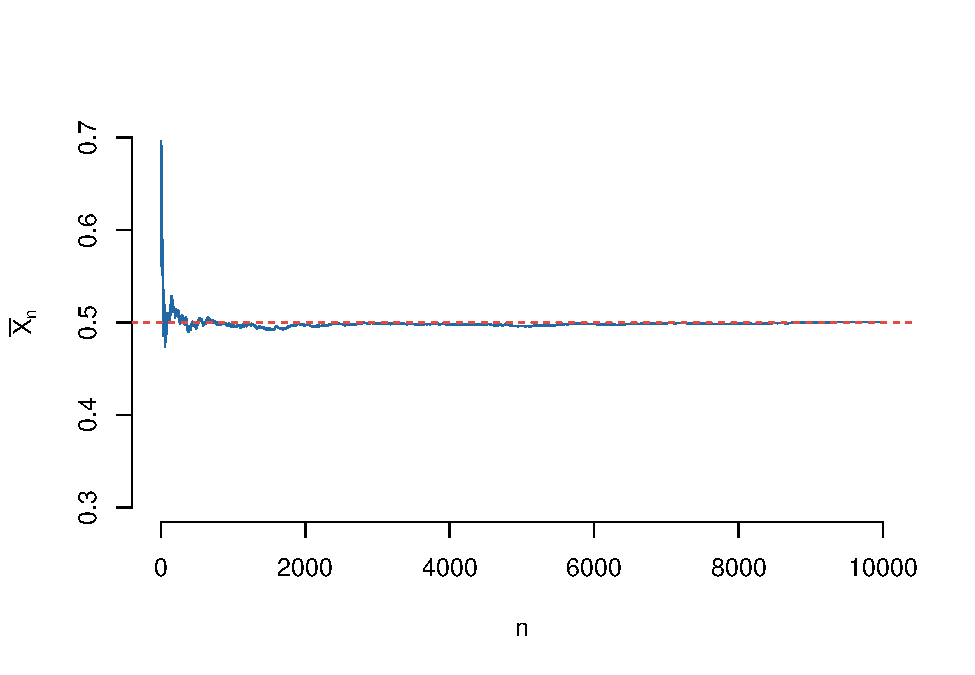
\includegraphics[width=0.7\linewidth]{Lab7_files/figure-latex/unnamed-chunk-8-1} \end{center}

În cazul în care v.a. \(X_1,X_2,\dots,X_N\) sunt normale de parametrii
\(\mathcal{N}(2,1)\) (deci media este \(\mu=2\)) avem:

\begin{Shaded}
\begin{Highlighting}[]
\CommentTok{# Folosim acelasi numar de variabile n}

\CommentTok{# Pentru legea normala folosim comanda rnorm}
\CommentTok{# Pentru calculul sumelor partiale putem folosi functia cumsum}
\NormalTok{y2 =}\StringTok{ }\KeywordTok{cumsum}\NormalTok{(}\KeywordTok{rnorm}\NormalTok{(n, }\DataTypeTok{mean =} \DecValTok{2}\NormalTok{, }\DataTypeTok{sd =} \DecValTok{1}\NormalTok{))}
\NormalTok{y2 =}\StringTok{ }\NormalTok{y2}\OperatorTok{/}\NormalTok{(}\DecValTok{1}\OperatorTok{:}\NormalTok{n)}
\NormalTok{mu2 =}\StringTok{ }\DecValTok{2} \CommentTok{# media normalei N(2,1)}

\CommentTok{# facem graficul }
\NormalTok{mar.default <-}\StringTok{ }\KeywordTok{c}\NormalTok{(}\DecValTok{5}\NormalTok{,}\DecValTok{4}\NormalTok{,}\DecValTok{4}\NormalTok{,}\DecValTok{2}\NormalTok{) }\OperatorTok{+}\StringTok{ }\FloatTok{0.1}
\KeywordTok{par}\NormalTok{(}\DataTypeTok{mar =}\NormalTok{ mar.default }\OperatorTok{+}\StringTok{ }\KeywordTok{c}\NormalTok{(}\DecValTok{0}\NormalTok{, }\FloatTok{0.3}\NormalTok{, }\DecValTok{0}\NormalTok{, }\DecValTok{0}\NormalTok{)) }
\KeywordTok{plot}\NormalTok{(}\DecValTok{1}\OperatorTok{:}\NormalTok{n, y2, }\DataTypeTok{type =} \StringTok{"l"}\NormalTok{, }
     \DataTypeTok{col=}\NormalTok{ myblue, }\DataTypeTok{xlab =} \StringTok{"n"}\NormalTok{, }
     \DataTypeTok{ylab =} \KeywordTok{expression}\NormalTok{(}\KeywordTok{bar}\NormalTok{(X)[n]),}
     \DataTypeTok{bty =} \StringTok{"n"}\NormalTok{,}
     \DataTypeTok{ylim =} \KeywordTok{c}\NormalTok{(}\FloatTok{1.5}\NormalTok{, }\FloatTok{2.5}\NormalTok{))}
\KeywordTok{abline}\NormalTok{(}\DataTypeTok{h =}\NormalTok{ mu2, }\DataTypeTok{col =}\NormalTok{ myred, }\DataTypeTok{lty=} \StringTok{"dashed"}\NormalTok{) }\CommentTok{# adaugam linia orizontala}
\end{Highlighting}
\end{Shaded}

\begin{center}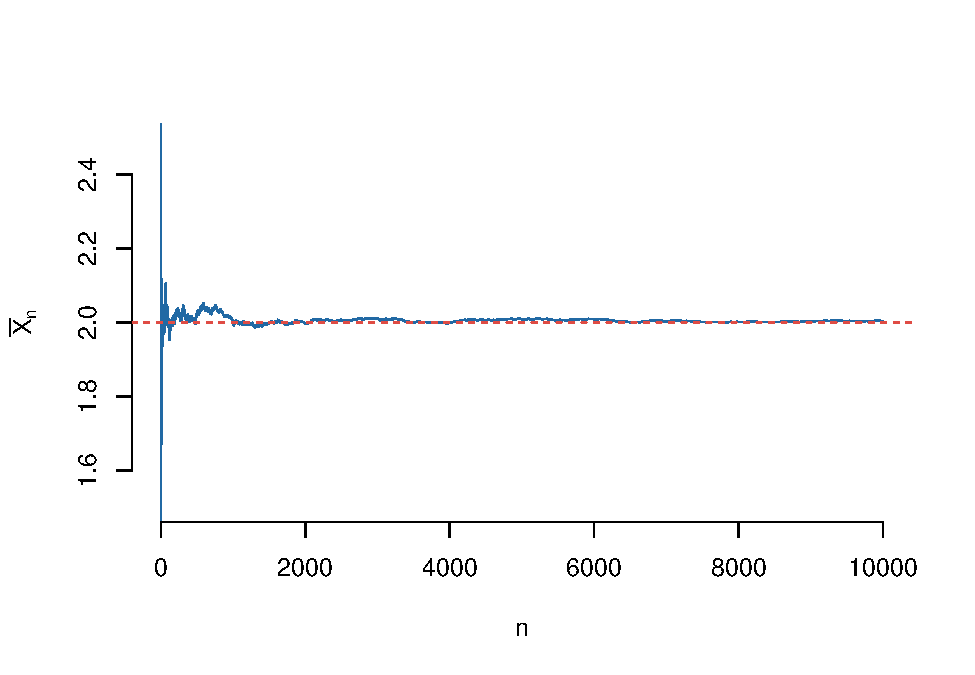
\includegraphics[width=0.7\linewidth]{Lab7_files/figure-latex/unnamed-chunk-9-1} \end{center}

\begin{rmdexercise}
Construiți o funcție care să vă permită generarea a \(m\) eșantioane de
volum \(n\) dintr-o populație normală de medie \(\mu\) și varianță
\(\sigma^2\) dată. Ilustrați grafic cu ajutorul unui boxplot cum variază
diferența dintre media aritmetică (media eșantionului \(\bar{X}_n\)) și
media teoretică pentru \(m = 100\) și diferite volume ale eșantionului
\(n\in\{10, 100, 1000, 10000\}\). Se consideră \(\mu = 1\) și
\(\sigma^2 = 1\).
\end{rmdexercise}

Următoarea funcție verifică cerința din problemă
(\texttt{normal.mean\ =} \(\mu\), \texttt{normal.sd\ =} \(\sigma\),
\texttt{num.samp\ =\ m} și \texttt{samp.size\ =\ n}). Să observăm că am
folosit funcția \texttt{rowMeans} pentru a calcula media fiecărui
eșantion (media pe liniile matricii de observații).

\begin{Shaded}
\begin{Highlighting}[]
\NormalTok{normalSampleMean <-}\StringTok{ }\ControlFlowTok{function}\NormalTok{(normal.mean, normal.sd, num.samp, samp.size) \{}
  \CommentTok{# generam matricea de observatii }
\NormalTok{    x =}\StringTok{ }\KeywordTok{matrix}\NormalTok{(}\KeywordTok{rnorm}\NormalTok{(}\DataTypeTok{n =}\NormalTok{ num.samp }\OperatorTok{*}\StringTok{ }\NormalTok{samp.size, }\DataTypeTok{mean =}\NormalTok{ normal.mean, }\DataTypeTok{sd =}\NormalTok{ normal.sd), }
        \DataTypeTok{nrow =}\NormalTok{ num.samp, }\DataTypeTok{ncol =}\NormalTok{ samp.size)}
    
  \CommentTok{# calculam media esantionului pentru fiecare esantion}
\NormalTok{    x.mean =}\StringTok{ }\KeywordTok{rowMeans}\NormalTok{(x)}
    
    \KeywordTok{return}\NormalTok{(x.mean)}
\NormalTok{\}}
\end{Highlighting}
\end{Shaded}

Pentru a ilustra grafic să considerăm o populație \(\mathcal{N}(1,1)\)
și pentru talie a eșantionului, \(n\in\{10, 100, 1000, 10000\}\), să
calculăm \(\bar{X}_n\) corespunzător (aici am folosit funcția
\texttt{sapply} - a se vedea laboratorul 3).

\begin{Shaded}
\begin{Highlighting}[]
\CommentTok{# date de intrare}
\NormalTok{normal.mean =}\StringTok{ }\DecValTok{1}
\NormalTok{normal.sd =}\StringTok{ }\DecValTok{1}
\NormalTok{true.mean =}\StringTok{ }\NormalTok{normal.mean}

\CommentTok{# marimea esantioanelor}
\NormalTok{samp.sizes =}\StringTok{ }\KeywordTok{c}\NormalTok{(}\DecValTok{10}\NormalTok{, }\DecValTok{100}\NormalTok{, }\DecValTok{1000}\NormalTok{, }\DecValTok{10000}\NormalTok{)}

\KeywordTok{names}\NormalTok{(samp.sizes) =}\StringTok{ }\KeywordTok{paste0}\NormalTok{(}\StringTok{"n = "}\NormalTok{, samp.sizes)}

\CommentTok{# numarul de esantioane}
\NormalTok{num.samp =}\StringTok{ }\DecValTok{100}

\CommentTok{# calculul mediei de selectie pentru fiecare esantion}
\NormalTok{x.mean =}\StringTok{ }\KeywordTok{sapply}\NormalTok{(samp.sizes, normalSampleMean, }\DataTypeTok{num.samp =}\NormalTok{ num.samp, }
                \DataTypeTok{normal.mean =}\NormalTok{ normal.mean, }\DataTypeTok{normal.sd =}\NormalTok{ normal.sd)}

\CommentTok{# ilustrarea grafica}
\NormalTok{mar.default <-}\StringTok{ }\KeywordTok{c}\NormalTok{(}\DecValTok{5}\NormalTok{,}\DecValTok{4}\NormalTok{,}\DecValTok{4}\NormalTok{,}\DecValTok{2}\NormalTok{) }\OperatorTok{+}\StringTok{ }\FloatTok{0.1}
\KeywordTok{par}\NormalTok{(}\DataTypeTok{mar =}\NormalTok{ mar.default }\OperatorTok{+}\StringTok{ }\KeywordTok{c}\NormalTok{(}\DecValTok{0}\NormalTok{, }\FloatTok{0.2}\NormalTok{, }\DecValTok{0}\NormalTok{, }\DecValTok{0}\NormalTok{), }\DataTypeTok{bty =} \StringTok{"n"}\NormalTok{) }
\KeywordTok{boxplot}\NormalTok{(x.mean }\OperatorTok{-}\StringTok{ }\NormalTok{true.mean, }
        \DataTypeTok{xlab =} \StringTok{"Talia esantionului (n)"}\NormalTok{, }
        \DataTypeTok{ylab =} \KeywordTok{expression}\NormalTok{(}\KeywordTok{bar}\NormalTok{(X)[n] }\OperatorTok{-}\StringTok{ }\NormalTok{mu),}
        \DataTypeTok{col =} \StringTok{"gray80"}\NormalTok{,}
        \DataTypeTok{bty =} \StringTok{"n"}\NormalTok{)}

\KeywordTok{abline}\NormalTok{(}\DataTypeTok{h =} \DecValTok{0}\NormalTok{, }\DataTypeTok{lty =} \DecValTok{2}\NormalTok{, }\DataTypeTok{col =}\NormalTok{ myred)}
\end{Highlighting}
\end{Shaded}

\begin{center}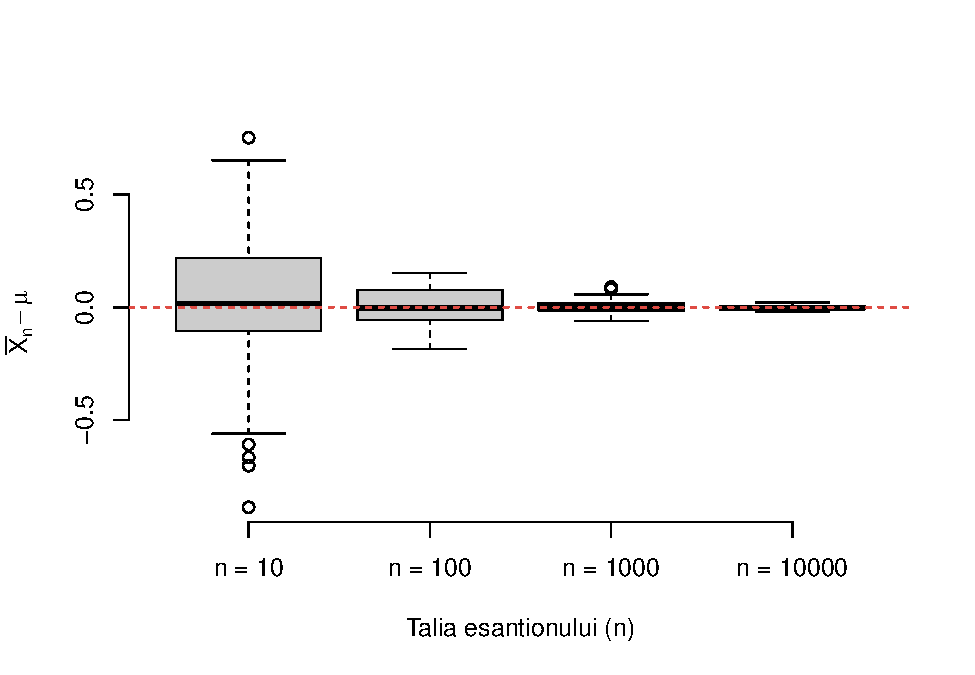
\includegraphics[width=0.7\linewidth]{Lab7_files/figure-latex/unnamed-chunk-12-1} \end{center}

Din boxplot-ul de mai sus observăm că pe măsură ce creștem talia
eșantionului media boxplot-ului se duce spre 0 ceea ce justifică enunțul
\emph{Legii Numerelor Mari}, și anume că media eșantionului converge la
media populației (media teoretică). De asemenea putem observa că și
varianța scade (gradul de împrăștiere scade) odată cu creșterea
numărului de observații.

\begin{rmdexercise}
Utilizați \emph{Legea Numerelor Mari} pentru a aproxima integrala
următoare

\[
  I = \int_{0}^{1}e^{x}sin(2x)cos(2x)dx.
\]

Calculați de asemenea valoarea exactă \(I\) a acesteia și comparați-o cu
aproximarea găsită.
\end{rmdexercise}

Fie \(U_1,U_2,\dots,U_n\) un șir de v.a. i.i.d. repartizare uniform pe
\([0,1]\). Cum \(g\) este o funcție continuă atunci
\(g(U_1), g(U_2),\ldots, g(U_n)\) sunt variabile aleatoare i.i.d. și
aplicând \emph{Legea Numerelor Mari} obținem

\[
  g_n=\frac{1}{n}\sum_{i=1}^{n}g(U_{i}) \overset{\mathbb{P}}{\to} \mathbb{E}[g(U_1)] = \int_{0}^{1}g(x)dx.
\]

Pentru a calcula integrala numeric vom folosi funcția \texttt{integrate}
(trebuie observat că această integrală se poate calcula ușor și exact
prin integrare prin părți). Următorul script ne dă valoare numerică și
aproximarea obținută cu ajutorul metodei Monte Carlo pentru integrale
\(\int_{0}^{1}g(x)dx\):

\begin{Shaded}
\begin{Highlighting}[]
\NormalTok{myfun=}\ControlFlowTok{function}\NormalTok{(x)\{}
\NormalTok{  y =}\StringTok{ }\KeywordTok{exp}\NormalTok{(x)}\OperatorTok{*}\KeywordTok{sin}\NormalTok{(}\DecValTok{2}\OperatorTok{*}\NormalTok{x)}\OperatorTok{*}\KeywordTok{cos}\NormalTok{(}\DecValTok{2}\OperatorTok{*}\NormalTok{x);}
  \KeywordTok{return}\NormalTok{(y);}
\NormalTok{\}}

\CommentTok{# calculul integralei cu metode numerice}
\NormalTok{I =}\StringTok{ }\KeywordTok{integrate}\NormalTok{(myfun,}\DecValTok{0}\NormalTok{,}\DecValTok{1}\NormalTok{) }\CommentTok{# raspunsul este o lista si oprim prima valoare}
\NormalTok{I =}\StringTok{ }\NormalTok{I[[}\DecValTok{1}\NormalTok{]]}

\CommentTok{# calculul integralei cu ajutorul metodei Monte Carlo}
\NormalTok{n =}\StringTok{ }\DecValTok{10000} 

\NormalTok{u =}\StringTok{ }\KeywordTok{runif}\NormalTok{(n) }\CommentTok{# generarea sirului U_n}
\NormalTok{z =}\StringTok{ }\KeywordTok{myfun}\NormalTok{(u) }\CommentTok{# calcularea sirului g_n}

\NormalTok{I2 =}\StringTok{ }\KeywordTok{sum}\NormalTok{(z)}\OperatorTok{/}\NormalTok{n }\CommentTok{# aproximarea MC}
\end{Highlighting}
\end{Shaded}

Obținem că valoarea numerică a lui \(I\) este 0.2662 iar cea obținută cu
ajutorul metodei Monte Carlo este 0.2673.

Avem următoarea ilustrare grafică a convergenței metodei Monte Carlo:

\begin{Shaded}
\begin{Highlighting}[]
\CommentTok{# graficul}
\NormalTok{gn =}\StringTok{ }\KeywordTok{myfun}\NormalTok{(}\KeywordTok{runif}\NormalTok{(n)) }
\NormalTok{gn =}\StringTok{ }\KeywordTok{cumsum}\NormalTok{(gn)}\OperatorTok{/}\NormalTok{(}\DecValTok{1}\OperatorTok{:}\NormalTok{n) }\CommentTok{# calculul lui g_n}

\KeywordTok{plot}\NormalTok{(}\DecValTok{1}\OperatorTok{:}\NormalTok{n, gn, }\DataTypeTok{type =} \StringTok{"l"}\NormalTok{, }
     \DataTypeTok{col =}\NormalTok{ myblue, }\DataTypeTok{xlab =} \StringTok{"n"}\NormalTok{, }
     \DataTypeTok{ylab =} \KeywordTok{expression}\NormalTok{(g[n]),}
     \DataTypeTok{bty =} \StringTok{"n"}\NormalTok{,}
     \DataTypeTok{ylim =} \KeywordTok{c}\NormalTok{(I}\OperatorTok{-}\FloatTok{0.2}\NormalTok{, I}\OperatorTok{+}\FloatTok{0.2}\NormalTok{))}
\KeywordTok{abline}\NormalTok{(}\DataTypeTok{h =}\NormalTok{ I, }\DataTypeTok{lty =} \StringTok{"dashed"}\NormalTok{, }\DataTypeTok{col =}\NormalTok{ myred)}
\end{Highlighting}
\end{Shaded}

\begin{center}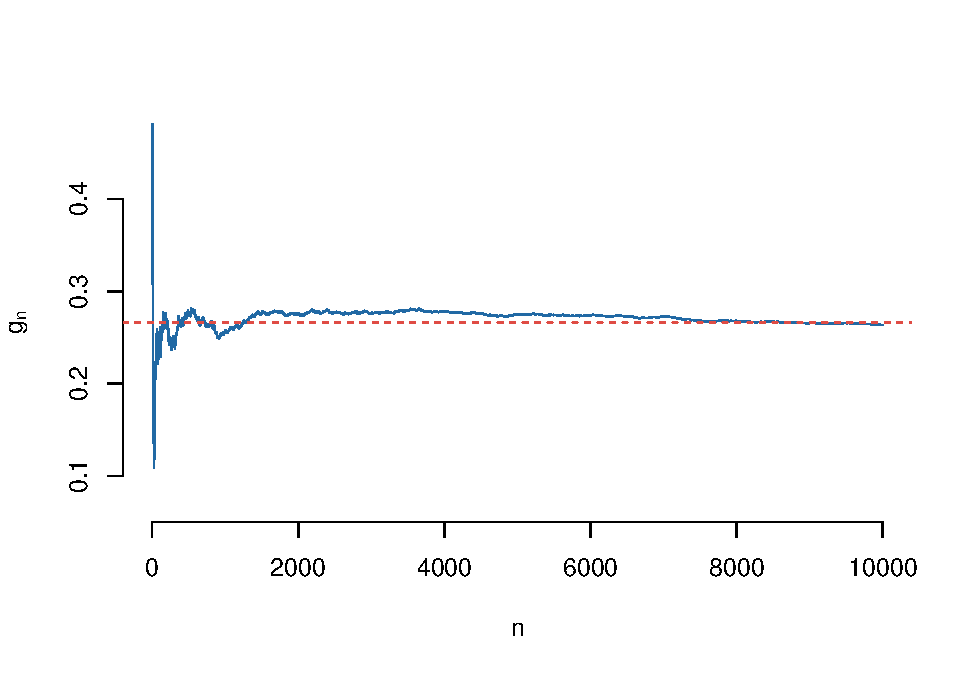
\includegraphics[width=0.7\linewidth]{Lab7_files/figure-latex/unnamed-chunk-15-1} \end{center}

\section{Ilustrarea Teoremei Limită
Centrală}\label{ilustrarea-teoremei-limita-centrala}

\begin{rmdinsight}
Fie \(X_1, X_2, \ldots\) un șir de variabile aleatoare independente și
indentic repartizate, de medie \(\mathbb{E}[X_1] = \mu<\infty\) și
varianță \(Var(X_1) = \sigma^2<\infty\). Atunci, notând
\(S_n = X_1 + \cdots + X_n\), avem

\[
  \mathbb{P}\left(\frac{S_n - \mathbb{E}[S_n]}{\sqrt{Var(S_n)}}\leq x\right) = \mathbb{P}\left(\frac{S_n - n\mu}{\sigma\sqrt{n}}\leq x\right) \overset{n\to\infty}{\longrightarrow} \Phi(x) = \frac{1}{\sqrt{2\pi}}\int_{-\infty}^{x}e^{-\frac{t^2}{2}}\,dt, \quad \forall x\in\mathbb{R}.
\]

Echivalent, dacă notăm media eșantionului cu
\(\bar{X}_n = \frac{S_n}{n}\), atunci

\[
  \mathbb{P}\left(\sqrt{n}\frac{\bar{X}_n - \mu}{\sigma}\leq x\right) \overset{n\to\infty}{\longrightarrow} \Phi(x) = \frac{1}{\sqrt{2\pi}}\int_{-\infty}^{x}e^{-\frac{t^2}{2}}\,dt, \quad \forall x\in\mathbb{R}.
\]
\end{rmdinsight}

\begin{rmdexercise}
Să presupunem că primim o monedă și ni se spune că aceasta aterizează pe
fața cap în \(48\%\) din cazuri. Vrem să testăm această afirmație.
Folosind \emph{Teorema Limită Centrală} și știind că vrem să fim siguri
în \(95\%\) din cazuri, ne întrebăm de câte ori trebuie să aruncăm
moneda pentru a verifica afirmația? Comparați răspunsul cu cel din
exercițiul în care am folosit \emph{LNM}, de mai sus.
\end{rmdexercise}

Folosind aceleași notații ca și în exercițiul din secțiunea de mai sus
și notând în plus \(S_n = X_1+\cdots+X_n\), avem

\begin{align*}
  \mathbb{P}\left(\frac{S_n}{n}<0.5\right) &= \mathbb{P}\left(\frac{S_n - n\mu}{\sigma\sqrt{n}}<\frac{(0.5-\mu)\sqrt{n}}{\sigma}\right)= \mathbb{P}\left(\frac{S_n - n\mu}{\sigma\sqrt{n}}<\frac{0.02\sqrt{n}}{\sqrt{0.2496}}\right) \\
  &= \mathbb{P}\left(\frac{S_n - n\mu}{\sigma\sqrt{n}}<0.04\sqrt{n}\right) \approx\Phi(0.04\sqrt{n})\geq 0.95
\end{align*}

Prin urmare, \((0.04\sqrt{n}\geq 1.645\) de unde \(n = 1692\). Putem
observa că rezultatul obținut prin aplicarea \emph{Teoremei Limită
Centrală} este mai precis decât cel obținut prin aplicarea \emph{Legii
numerelor mari}.

\begin{rmdexercise}
Fie \((X_n)_{n\geq1}\) un șir de v.a. i.i.d. de lege \(\mathcal{E}(1)\).
Pentru toți \(n\), notăm cu \(S_n=X_1+X_2+\cdots X_n\) șirul sumelor
parțiale, \(\mu\) și \(\sigma^2\) reprezentând media și respectiv
varianța legii \(\mathcal{E}(1)\). \emph{Teorema Limită Centrală} afirmă
că dacă \(n\) este mare atunci v.a.

\[
\frac{S_n-n\mu}{\sqrt{n}\sigma}
\]

are aproximativ aceeași distribuție ca și legea normală
\(\mathcal{N}(0,1)\). Ilustrați această convergență în distribuție cu
ajutorul unei histograme. Suprapuneți peste această histogramă
densitatea legii \(\mathcal{N}(0,1)\).
\end{rmdexercise}

Știm că media unei v.a. distribuite exponențial de parametru
\(\lambda\), \(\mathcal{E}(\lambda)\) este \(\mu=\frac{1}{\lambda}\) iar
varianța acesteia este \(\sigma^2=\frac{1}{\lambda^2}\). Pentru fiecare
valoare a lui \(i\) de la \(1\) la \(N\) calculăm raportul
\(\frac{S_n-n\mu}{\sigma\sqrt{n}}\) (cu alte cuvinte repetăm
experimentul de \(N\) ori):

\begin{Shaded}
\begin{Highlighting}[]
\NormalTok{N =}\StringTok{ }\DecValTok{1000} \CommentTok{# alegem numarul de repetitii ale experimentului}
\NormalTok{n =}\StringTok{ }\DecValTok{1000} \CommentTok{# alegem n pentru care folosim aproximarea normala}

\NormalTok{lambda =}\StringTok{ }\DecValTok{1} \CommentTok{# parametrul legii E(1)}

\NormalTok{mu =}\StringTok{ }\DecValTok{1}\OperatorTok{/}\NormalTok{lambda }\CommentTok{# media}
\NormalTok{sigma =}\StringTok{ }\DecValTok{1}\OperatorTok{/}\NormalTok{lambda }\CommentTok{# abaterea standard }

\NormalTok{s =}\StringTok{ }\KeywordTok{rep}\NormalTok{(}\DecValTok{0}\NormalTok{,N) }\CommentTok{# initializam sirul sumelor partiale}

\ControlFlowTok{for}\NormalTok{ (i }\ControlFlowTok{in} \DecValTok{1}\OperatorTok{:}\NormalTok{N)\{}
\NormalTok{  x =}\StringTok{ }\KeywordTok{rexp}\NormalTok{(n, }\DataTypeTok{rate =}\NormalTok{ lambda) }\CommentTok{# generam variabilele exponentiale}
\NormalTok{  s[i] =}\StringTok{ }\NormalTok{(}\KeywordTok{sum}\NormalTok{(x)}\OperatorTok{-}\NormalTok{n}\OperatorTok{*}\NormalTok{mu)}\OperatorTok{/}\NormalTok{(sigma}\OperatorTok{*}\KeywordTok{sqrt}\NormalTok{(n)) }\CommentTok{# calculam raportul }
  
\NormalTok{\}}
\end{Highlighting}
\end{Shaded}

Continuăm prin trasarea histogramei cerute și adăugăm la grafic
densitatea legii normale \(\mathcal{N}(0,1)\):

\begin{Shaded}
\begin{Highlighting}[]
\CommentTok{# trasam histograma}
\CommentTok{# pentru mai multe optiuni latex: ?plotmath }
\KeywordTok{hist}\NormalTok{(s, }\DataTypeTok{main =} \KeywordTok{expression}\NormalTok{(}\KeywordTok{paste}\NormalTok{(}\StringTok{"Histograma raportului "}\NormalTok{,}
                                \KeywordTok{frac}\NormalTok{(S[n]}\OperatorTok{-}\NormalTok{n}\OperatorTok\NormalTok{mu,sigma}\OperatorTok\KeywordTok{sqrt}\NormalTok{(n)))),}
     \DataTypeTok{prob =} \OtherTok{TRUE}\NormalTok{, }
     \DataTypeTok{col =} \StringTok{"grey80"}\NormalTok{, }\CommentTok{# Culoarea de umplere}
     \DataTypeTok{border =} \StringTok{"grey20"}\NormalTok{,}
     \DataTypeTok{xlim =} \KeywordTok{c}\NormalTok{(}\OperatorTok{-}\DecValTok{4}\NormalTok{,}\DecValTok{4}\NormalTok{), }
     \DataTypeTok{cex.main=}\FloatTok{0.75}\NormalTok{, }
     \DataTypeTok{cex.lab =} \FloatTok{0.75}\NormalTok{, }
     \DataTypeTok{cex.axis =} \FloatTok{0.75}\NormalTok{, }
     \DataTypeTok{xlab =} \StringTok{""}\NormalTok{, }
     \DataTypeTok{ylab =} \StringTok{"Densitatea"}\NormalTok{)}

\CommentTok{# adaugam densitatea normalei N(0,1) }
\NormalTok{x1 =}\StringTok{ }\KeywordTok{seq}\NormalTok{(}\OperatorTok{-}\DecValTok{4}\NormalTok{,}\DecValTok{4}\NormalTok{,}\DataTypeTok{by=}\FloatTok{0.1}\NormalTok{)}
\NormalTok{y1 =}\StringTok{ }\KeywordTok{dnorm}\NormalTok{(x1, }\DataTypeTok{mean =} \DecValTok{0}\NormalTok{, }\DataTypeTok{sd =} \DecValTok{1}\NormalTok{)}
\KeywordTok{lines}\NormalTok{(x1, y1, }\DataTypeTok{col =}\NormalTok{ myred, }\DataTypeTok{lwd =} \DecValTok{2}\NormalTok{, }\DataTypeTok{lty =} \DecValTok{2}\NormalTok{)}
\end{Highlighting}
\end{Shaded}

\begin{center}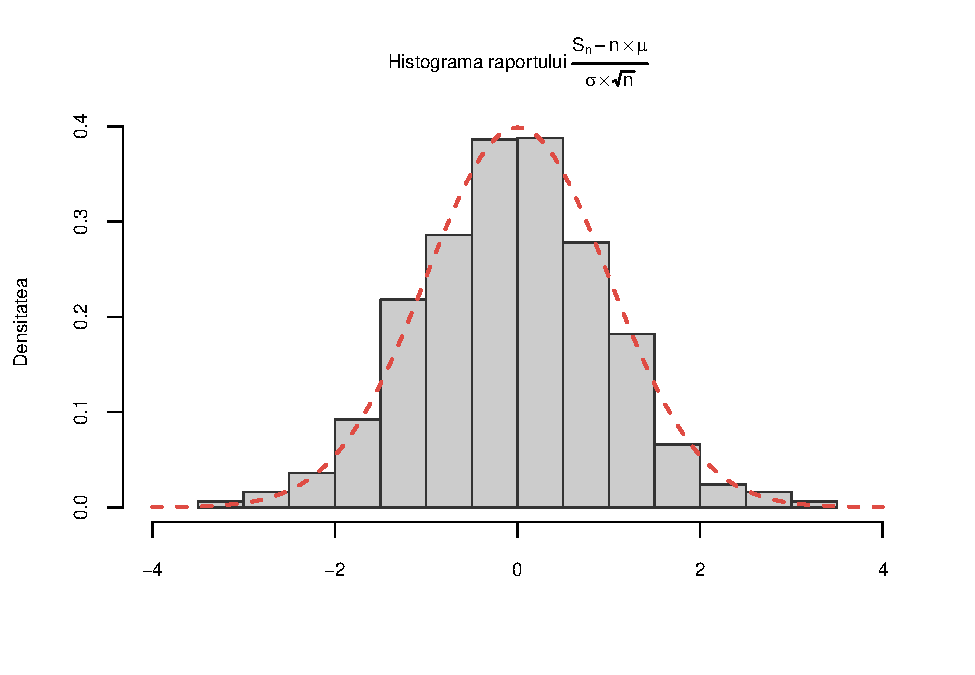
\includegraphics[width=0.7\linewidth]{Lab7_files/figure-latex/unnamed-chunk-20-1} \end{center}


\end{document}
